\section{Phospholipid bilayers}
Phospholipid bilayers are the primary component of the major delimiting boundary between cells and their environment.
These membranes are not static walls so much as liquid-crystalline, rapidly exploring their conformational
space and adjusting to the external and internal cellular environment. Cells, through the 
diversity of chemistry of headgroups and acyl-chain selections, tailor the dynamic structure of their membrane to further
adapt to the environment around them. 
Understanding the way that individual lipid species contribute to the structure of a lipid bilayer is critical to understand
why a cell might choose one lipid or another in their cell membrane. Additionally, because these lipids are exposed to complex
mixtures of ions on either side of the membrane, the interactions with ions in solution cannot be ignored when discussing the bilayer structure. 
Experimentally observed ion behavior at an interface in solution has been explained using a mean-field model~\cite{israelachvilli:2011:intermol}.
However, this ignores specific chemical interactions between lipid molecules and the ions in the solvent, that are critical for understanding
the effect of changing headgroup species in a membrane. 
Computational models can enable researchers to observe the specific ion-lipid interactions are critical for understanding of 
why cells might choose certain lipids to manipulate their membrane structure under varied ion mixtures in their environment. Furthermore, this 
changing membrane structure also affects the behavior of membrane protiens embedded in the bilayer. Thus, this manipulation of the lipid mixture
presents itself as an important regulatory mechanism for cells.
\subsection{Effects of ions on lipid bilayer structure}
The effects of dissolved salts on bilayers has been studied with varied methodologies. 
One of the more commonly applied methods of study
is small-angle x-ray scattering (SAXS) and neutron scattering (SANS). 
Several studies of this kind havereported
largely that salts do not have a significant affect on zwitterionic lipid bilayer 
structure~\cite{pabst:2007,petrache:2006:swelling,uhrikova:2008,kurakin:2021:effect}.
Petrache \etal{} observed that with multilamellar vesicles of 1,2-dilauroyl-sn-glycero-3-sn-glycero-phosphatidylcholine 
as well as other lipids in KCl and BrCl salt solutions, 
and reported that while small changes can be seen in the
X-ray scattering form-factor due to the 
salts, 
the fitted electron density profiles are essentially identical for
systems with and without 
salt~\cite{petrache:2006:swelling}. 
Similarly, Pabst \etal{} found no significant change in bilayer structure 
for POPC bilayers in NaCl salt at or below 1 M concentration~\cite{pabst:2007}.
Furthermore, Uhrikova \etal{} reported small structural changes using small angle neutron scattering
(SANS) experiments on 1,2-dipalmitoyl-sn-glycero-3-phosphatidylcholine 
vesicles interacting with CaCl$_{2}$~\cite{uhrikova:2008}. 
Taken together, these results point to a general discrepancy between structural data 
from MD simulations and scattering experiments.
Kurakin \etal{} reported that in bilayers of POPC, divalent cations such as \mg{} and Ca\textsuperscript{2+} also cause
no major alteration in lipid bilayer structure at biologically relevant concentrations of \mg~\cite{kurakin:2021:effect}.

While SAXS and SANS methods do not see a change in the overall structure of lipid bilayers methods like NMR of deuterated headgroup carbons 
indicate changes in the headgroup tilt angle of neutral lipids in salt solutions, suggesting some interaction~\cite{akutsu:1981,seelig:1987}. 
This would indicate that there should be ion binding or adsorption to the bilayer interface, that is not visible in the SAXS or SANS form-factor but 
could be observed through other methods. Additionally, AFM measurements can observe some changes in the organization of lipids in a 
gel phase bilayer in the presence of salts, again indicating some interaction 
and adsorption while the area-per-lipid of the bilayer remains largely unchanged~\cite{ferber:2011:direct}.

Molecular simulations can gather atomistic detail of systems, and are often useful for systems like lipid bilayers. Simulations of bilayers
in salt using many different simulation models 
have reported that there is significant ion binding to the lipid bilayer, and subsequent 
thickening of the lipid bilayer when compared to the structure 
of a bilayer in pure 
water~\cite{Bockmann:2003,cordomi:2008,gurtovenko:2008,Cordomi:2009,jurkiewicz:2012,pandit:2008:simulationtextbook,kruczek:2017,kruczek:2019,saunders:2019}.
This persistent discrepancy between the large-scale structural changes predicted by 
simulations and the subtle rearrangements observed experimentally highlights the need for improved 
ion-lipid interaction models that better capture experimental behavior. 
In the following chapters, this problem is addressed through the development of a generalizable 
method for selecting molecular simulation parameters to reproduce target experimental data, and through 
the application of this method to refine lipid-ion interaction models across a range of salt solutions. 
The remainder of this introduction outlines the simulation and analysis methods employed throughout this work, 
while the subsequent chapters present the specific results obtained.


\section{Molecular Simulations}
\subsection{Classical Molecular Dynamics}
Molecular Dynamics utilizes computers to simulate systems of molecules in order to study how structure changes
with time, and the specific ways that different atomic and molecular species interact. This is done
by first creating a model for the Hamiltonian of the system --- a ``force-field''. This consists firstly of the terms for how atoms
bond to each other, how these bonds move and stretch, and how they rotate around each other; classical models
usually use harmonic potentials for bond and angle stretching and bending, and dihedrals 
are described using periodic functions~\cite{gromacsmanual}.
In addition to the bonded terms, we have the non-bonded terms — energy from 
electrostatic interactions, typically described by Coulomb's law, and dispersion 
interactions (Van der Waals, or VdW) which arise from instantaneous dipole-induced dipole effects~\cite{gromacsmanual}. These are 
most often modeled using a Lennard-Jones (LJ) potential~\cite{Jones:1924,gromacsmanual}, though other forms are 
also common, such as the Buckingham (exp-6) potential~\cite{Buckingham:1938,gromacsmanual}, which replaces the steep 
\(r^{-12}\) repulsive wall with a short-range exponential. In addition to these two, there are many other
functional forms used to describe VdW and dispersion interactions, but they are far less common. An example of this Hamiltonian
can be seen here:
\begin{align}
E_{\mathrm{total}} &= E_{\mathrm{bonded}} + E_{\mathrm{nonbonded}} \\
E_{\mathrm{bonded}} &= \sum_{\text{bonds}} k_r (r - r_0)^2
+ \sum_{\text{angles}} k_\theta (\theta - \theta_0)^2
+ \sum_{\text{dihedrals}} V_n \left[ 1 + \cos\left( n\phi - \gamma \right) \right] \\
E_{\mathrm{nonbonded}} &= \sum_{i<j} \left[ 4\epsilon_{ij} \left( \left( \frac{\sigma_{ij}}{r_{ij}} \right)^{12}
- \left( \frac{\sigma_{ij}}{r_{ij}} \right)^{6} \right)
+ \frac{q_i q_j}{4\pi\epsilon_0 r_{ij}} \right]
\end{align}

By using this set of terms one can compute the potential energy of a particular configuration of particles. 
The forces obtained from the potential energy are used in Newton's equations of motion, 
which are numerically integrated — most often with algorithms such as the velocity-Verlet method — 
to update positions and velocities at each time step~\cite{gromacsmanual}.
The energy of the new configuration
can be computed, and the simulation continues. Thus, the careful development and improvement of a force-field is critical to 
reproduce valid results that can help us understand what is seen in experiments.

\subsection{Mixing rules, and NB-fix}
Focusing in particular on the non-bonded terms of the hamiltonian, and specifically the Lennard-Jones (LJ) function, we note that there are two
free parameters \sigmaij{} and \epsilonij{} between a particular pair of particles $i$ and $j$:
\begin{equation}
E_{\mathrm{LJ}_{ij}} = 4\epsilon_{ij} \left( \left( \frac{\sigma_{ij}}{r_{ij}} \right)^{12}
- \left( \frac{\sigma_{ij}}{r_{ij}} \right)^{6} \right)
\end{equation}
Where $r_{ij}$ is the distance between the two particles, \sigmaij{} is the characteristic distance of the Van der Waals interaction between the two species,
and \epsilonij{} is the characteristic energy of the interaction.
These parameters are generally determined for a particular species for the case of the self-interaction, or $\sigma_{ii}$ and $\epsilon_{ii}$.
In this case, they represent roughly the atomic radius, and the ``stickyness'' of the particle. These can then be combined with the 
$\sigma_{jj}$ and $\epsilon_{jj}$ from another species by using what are called mixing rules, developed to 
model the interaction radii and energy well-depth for interacting species~\cite{lorentz:1881,berthelot:1898}.
The Lorentz rule for computing the \sigmaij{} is simply the arithmetic mean of the self terms from the two species, and 
the Berthelot rule for computing the \epsilonij{} is the geometric mean of the self terms.
Modern works have often reported that these mixing rules fail
or behave unpredicatbly for more complicated species than the noble gases~\cite{fyta:2012,boda:2008:effects},
and abandonment of the mixing rules for specifically selected cross-terms can be beneficial to improving
force-fields~\cite{baker:2010:accurate,yoo:2012:improved,fyta:2012:ionic,mamatkulov:2013:force,venable:2013,
savelyev:2014:balancing,li:2015:representation,savelyev:2015:competition,jing:2017:study,reif:2017,wineman:2019}. This 
kind of correction is often called a ``non-bonded fix'' or NB-fix, which is a correction to the cross-terms of the species of interest 
in order to improve the reproduction of some experimental result.
In this dissertation, I expand on the idea of a NB-fix method to improve the modeling of the interactions of ions and phospholipid species.
However, the method proposed and characterize is general, and can be applied to other chemically diverse systems of interest.

\subsubsection{MD methods utilized in this dissertation}
In the following dissertation, unless otherwise specified, I perform all molecular dynamics simulations with the GROMACS software 
package~\cite{abraham:2015,pall:2014,van:2005,lindahl:2001,berendsen:1995,gromacs}.
I use the SPC/E model for all waters~\cite{spce}, and I describe lipid interactions
with the gromos43A1-S3 parameter set developed by our group in previous work~\cite{chiu:2009}.
System temperature is maintained at 300~K using the Nos\`e-Hoover thermostat
with a coupling constant of 0.5~ps~\cite{nose:1983}, and pressure is maintained
at 1~atm with the Parrinello-Rahman semiisotropic barostat using a coupling constant of 1.5~ps~\cite{parrinello:1981}.
All bonds are constrained with the P-LINCS algorithm, which allows the use of a 4~fs integration timestep~\cite{lincs}.
Equations of motion are integrated with the Verlet scheme, and neighbor lists are updated every 2 steps.
Electrostatic interactions are treated with the particle-mesh Ewald (PME) method~\cite{essmann:1995},
using a real-space cutoff of 1.6~nm and reciprocal grids of either
$56 \times 56 \times 224$ or $52 \times 52 \times 240$ cells,
together with 4th order B-spline interpolation.
Van der Waals interactions are calculated with a single cutoff of 1.6~nm.
\subsubsection{Simulation system construction}
All simulations systems unless otherwise noted are constructed by first creating a leaflet of 100 POPC lipids arranged
on a $10 \times 10$ grid with sufficient spacing to avoid chain overlap.
This leaflet is then reflected along the $z$--axis to generate the second
leaflet, producing a bilayer of 200 lipids. A solvent block is added by
placing 60,000 water molecules on a three-dimensional grid with excess spacing,
and a subset of water molecules is randomly replaced with ions to achieve a
starting concentration of 200~mM (see Table~\ref{tabch3:ions}).

Energy minimization is performed using the steepest-descents algorithm with a
force tolerance of 50~kJ~mol$^{-1}$~nm$^{-1}$. Electrostatic interactions are
treated with the particle-mesh Ewald (PME) method~\cite{essmann:1995}, using a
real-space cutoff of 1.6~nm, reciprocal grid spacing of 0.12~nm$^{-1}$, and
6th order B-spline interpolation. Van der Waals interactions are calculated
with a single cutoff of 1.6~nm. Neighbor searching is performed every 2 steps.

Following energy minimization, I relax the system with a constant-pressure
simulation at 290~K for 200~ps. Simulation systems are then annealled by heating the system above the
simulation run temperature, and then cooling down to the production temperature following the
specific procedure outlined in each following chapter.

\subsection{\emph{Ab initio} calculations and Density Functional Theory}
Classical force-fields are effective for simulating large-systems of particles where an explicit description of 
the electronic behavior is not critical to the understanding of how the particles behave. While this is a major 
approximation, it turns out to often be useful in studying biological structures like lipid membranes~\cite{berkowitz:2019}.
However, when preparing these classical models, we need to refer to more complicated theory in the form 
of quantum mechanical calculations. These calculations are used to set terms like the 
charge per particle in a molecule and to compare to the molecular structure predicted by our bonded-parameters.
\emph{Ab initio} quantum mechanical calculations include chemistry by explicitly describing the behavior of electrons to varied 
levels of accuracy depending on the kind of functional form used, and then the basis vectors used to describe the space.
Pertubation theory methods include electron correlation, which can be useful for assigning electrons to parts of a molecule. 
However, these methods quickly become expensive for systems with many electrons. Density functional theory, which treats the electrons 
with a mean-field approximation is often more computationally efficient and can thus be applied to larger systems.

\emph{Ab initio} methods are used in the works included in this dissertation to generate target data for 
model parameter optimization from geometry
optimizations and substitution energies of small ion-ligand clusters
using density functional theory (DFT) as implemented in
FHI-aims~\cite{fhiaims}. Initial cluster geometries are produced with
the molecular mechanics force field developed in our previous
work~\cite{kruczek:2017,saunders:2019} and then optimized at the DFT
level. I use the PBE0 functional~\cite{perdew:1996:generalized,adamo:1999:toward}
with Tkatchenko-Scheffler dispersion corrections~\cite{tkatchenko:2009},
a combination that has been benchmarked for ion-ligand clusters and shown
to reproduce experimental data and high-level quantum methods across a
range of chemistries~\cite{wineman:2019,wineman:2020:transferable,wineman:2020:improved}.
Geometry optimizations are first performed with the ``light'' basis set
and then refined with the ``really tight'' basis set provided in
FHI-aims. Optimizations are converged to 0.005~eV/\AA{} in forces and
$10^{-6}$~eV in total energy.  

Energies of optimized clusters are then used to compute substitution
energies, defined as the energy of exchanging water molecules
with headgroup analog ligands. The specific cluster sets and substitution
energy targets used for parameterization are described in the relevant
chapters.

\section{Comparing Molecular Simulations with Experimental Results}
\subsection{Bilayer Structural Parameters}
SAXS and SANS measurements yield structural information of crystalline systems.
Lipid bilayers are smectic crystals, and thus give scattering
patterns that look like concentric rings in reciprocal space --- these circles are the bilayer form-factor~\cite{nagle:2000}. This form-factor
is the reciprocal-space structure of the bilayer. 
However, a direct Fourier inversion cannot be performed due to the loss of phase information.
In order to produce the appropriate density distribution, one can approximate the number density of bilayer parts as gaussian functions, and 
compute the appropriate scattering density from that~\cite{nagle:2000,fogarty:2015}. This can then be transformed via a cosine transform
into a form-factor. The gaussians are then adjusted
until the resulting continuous form-factor fits the data from the experiment~\cite{nagle:2000,fogarty:2015}. These density histograms are then used to compute the various bilayer parameters.

In simulations, one can compute the number density histograms of the system components
directly from the trajectories, and thus the electron densities directly. Once the electron density of our system has been obtained
per nanosecond, the lipid bilayer centerpoint is determined by locating the minimum at the center of the 
histogram. This is symmetrized around the minimum at the center, and then averaged over many nanoseconds.
The bulk solvent value of the electron density is set to zero by subtracting this from the average histogram, and then a cosine transform is used 
to obtain the bilayer SAXS form-factor. SANS form-factors are obtained similarly, but by using the neutron-scattering length density --- instead of weighting the number density 
by the number of electrons per particle, this weights them by the scattering length of the specific nucleus.
These formfactors can be compared with the experimental data directly.

One can also use the electron density to directly obtain the peak-to-peak distance of the bilayer, \dhh{}, as one measure
of the bilayer thickness. 
The number density histograms are also used to compute the various bilayer thicknesses via probability densities
of the various system components. We compute the bilayer thickness \db{} and \dc{} by compiuting probability densities
for the solvent, and the lipid acyl chains respectively. We determine the Gibbs' dividing surface of these by finding the point in the interfacial region
where the area above the histogram is equal to below --- the distance from this point to the bilayer center is used as the respective bilayer thickness.
These measures are visualized in figure~\ref{figch1:thicknesses}.
\begin{figure}[h!tb]
    \caption[Diagram of bilayer thickness measurements]{Measurements of the bilayer thickness that are often obtained in experiments and reproduced in simulations. We see the electron density in (b) shown in red,
    with the characteristic minimum at the bilayer center and the two peaks that roughly localize the electron-dense phosphate moiety. The \dhh{} is taken as the distance between the two peaks,
    measuring the bilayer repeat distance. In (a), we see probability densities for water (green) and solvent (purple). We compute the gibbs' dividing surface for each of these densities by taking the area 
    above and below the curve, and selecting the position where they become equal. The distance from this to the center of the bilayer is half of the bilayer thickness \db{} or \dc{}.}
    \label{figch1:thicknesses}
    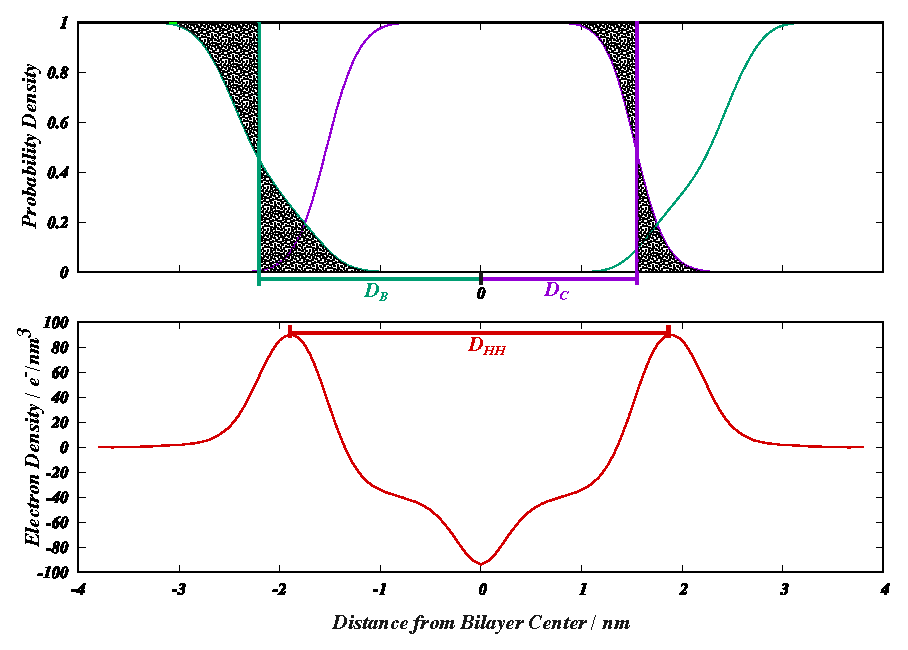
\includegraphics{Probabilitydens.eps}
\end{figure}
\subsubsection{Lipid component volumes}
Phospholipid headgroup and chain occupied volumes are computed using the method of Petrache \etal{} for computing the
volume of immiscible liquids~\cite{petrache:1997} using the number density histograms of the headgroups, acyl-chains, and solvent.
In the work outlined in this dissertation, we identify lipid chains are as starting 
at the first carbon attached to the lipid chain carbonyl oxygen, including the oxygen.
The atom groups not part of the lipid
chains are partitioned into the headgroup volume. 
The number-density of these component groups along with that of the solvent are taken 
and used to optimize the objective function:
\begin{equation}
    \label{eq:volumeobj}
    \Omega(v_i)=\sum^{\rho_s}_{z_j}(1-\sum^{N_{\text{Groups}}}_{i=1}{(\rho_i(z_j)v_i)^2})\text{,}
\end{equation}
In the equation above, $\rho_i(z_j)$ is the number density of the $i$ component in the
$z_j$ slice of the box and $v_i$ is the corresponding component volume. 
The component volumes are then multiplied by the corresponding
number of particles per molecule per group --- 32 for the chain
particles, and 20 for the headgroup. 
This gives us the total volume per molecule for each group, defined as \Vh{} and \Vc{}. These are then
added together to make the total \Vl{}.
\subsection{Deuterium Order parameters}
\subsubsection{D2O Water orientational order parameters}
Water ordering at the lipid bilayer interface can be measured by using NMR in a system minimally hydrated deuterium oxide~\cite{aaman:2003}.
The quadrupolar interaction of the deuterium nucleus with the magnetic field results in a splitting of the deuterium lineshape. The width of this splitting 
is used to make suppositions about the orientational ordering of water in the interfacial region --- this has a value of zero if the system is either isotropic or completely aligned with the
magnetic field, and takes non-zero values for any other average ordering.
In simulation, we compute 
orientational order parameters by defining the quadrupolar axis as the
OW$\rightarrow$HW1 bond of water, and the angle formed with the magnetic field director 
as that formed with the z-axis of the simulation box ($\beta$). 
These order parameters are defined using the first and second 
Legendre polynomials with respect to the angle $\beta$,
\begin{equation}
    \begin{split}
    P_1&=\langle \cos\left(\beta\right) \rangle
    \\ P_2&=\frac{1}{2}\bigg\langle\left(3\cos^2\left(\beta\right)-2\right)\bigg\rangle
    \text{,} 
\end{split}
\end{equation}
where average is over all the waters in a particular volume slice of the box 
and then over simulation time.  
We plot these values as a function of distance from the bilayer center. 
$P_1$ denotes dipolar ordering of the bond vector and the bilayer normal direction, 
with a positive value indicating an average outward orientation 
and a zero value corresponding to an average perpendicular orientation to the
bilayer normal or a uniformly random orientation. 
$P_2$ represents a nematic ordering, measuring more if the vector in question is more parallel to the box z-axis, with less regard to the directionality otherwise. This parameter 
is asymmetric around zero, with a zero value representing a vector that is completely parallel with the director axis. This second parameter is directly related to the quadrupolar splitting 
seen in experiments~\cite{aaman:2003,kruczek:2017:ether,saunders:2019}.
\subsubsection{Acyl-chain CD order parameters}
Similar to the water order parameters, lipid chain ordering can be determined experimentally by performing NMR 
on specifically deuterated hydrocarbon chains. Each C-D bond has a quadrupolar character from the deuterium nucleus, that results in
a quadrupolar splitting of the NMR spectral lineshape. The width of this splitting is directly related to the 
S\textsubscript{CD}, which changes with temperature and along the various thermodynamic phases of the lipid bilayer.

Since hydrogen/deuterium is not included on the coarse-grained lipid chains, 
one cannot directly access the C-D ordering by simply measuring the angle between the bond vector and the director field. 
Instead, one must compute the chain order tensor $S_{\alpha\beta}$ defined as
\begin{equation}
    S_{\alpha\beta}=\frac{1}{2}\big\langle
    3\cos{\theta_\alpha}\cdot\cos{\theta_\beta}-\delta_{\alpha\beta}\big\rangle,
    \nonumber
\end{equation}
where the angles $\theta_\alpha$ and $\theta_\beta$ are the angles between the molecular
axis and the box z-direction. 
Then use this tensor is used to calculate the $S_{CD}$ as
\begin{equation}
    -S_{CD}^{\text{Saturated}}=\frac{2}{3}S_{xx}+\frac{1}{3}S_{yy}
\end{equation}
for saturated carbons~\cite{egberts:1988}, and as
\begin{equation}
-S_{CD}^{\text{Unsaturated}}=\frac{1}{4}S_{zz}+\frac{3}{4}S_{yy}\mp \frac{\sqrt{3}}{2}S_{yz}
\end{equation}
for unsaturated carbons~\cite{Douliez:1995}.  
